\chapter{Considerações Finais} \label{cap:conclusao}

    O presente trabalho teve como objetivo principal analisar as vulnerabilidades presentes nas redes industriais que utilizam o protocolo OPC UA, abordando suas implicações de segurança e os riscos associados ao seu uso no contexto da Indústria 4.0.

\section{Conclusões}

    A primeira etapa da pesquisa consistiu em uma revisão detalhada sobre a arquitetura do OPC UA, abordando seus requisitos fundamentais, o funcionamento dos clientes e servidores OPC UA, bem como os procedimentos necessários para o estabelecimento de canais de comunicação seguros entre essas entidades. A partir dessa revisão, foi possível identificar diversas vulnerabilidades do protocolo, incluindo ataques de negação de serviço (DoS), escuta clandestina, falsificação de mensagens, alteração de mensagens, repetição de mensagens e sequestro de sessões.

    Em seguida, o trabalho propôs a implementação de um ambiente de testes baseado na arquitetura OPC UA, utilizando dispositivos Raspberry Pi para simular um cliente e um servidor OPC UA. Inicialmente, foi adotada a configuração padrão do protocolo, com a política de segurança definida como ``None''. No cenário experimental, três tipos de ataques cibernéticos foram realizados: sniffing de pacotes, ataque ``man in the middle'' (MITM) e ataque de negação de serviço (DoS). O ataque MITM, por exemplo, demonstrou a vulnerabilidade à comprometer a confidencialidade, a autorização e a autenticação da comunicação, evidenciando a dependência do tipo de configuração do open62541. Já os ataques DoS, realizados por meio de TCP-SYN Flood e TCP Anomalies, revelaram o impacto significativo desses ataques no uso da CPU do servidor OPC UA, com o TCP-SYN causando maior sobrecarga nos recursos computacionais.

    Além dos ataques, o trabalho também se concentrou em métodos de detecção simples, voltados para a identificação de tais ataques a partir do lado da vítima, utilizando ferramentas como Wireshark e ARP. Essa abordagem permitiu a identificação de padrões e anomalias associadas a ataques cibernéticos, proporcionando uma base para a prevenção e mitigação de falhas no sistema.

    As conclusões extraídas deste trabalho destacam a complexidade e a vulnerabilidade das redes industriais que utilizam o protocolo OPC UA. Embora amplamente adotado em diversos setores industriais, o protocolo apresenta sérias falhas de segurança que podem comprometer a integridade e a confidencialidade das comunicações. As vulnerabilidades identificadas neste estudo podem ter impactos graves nas operações industriais, especialmente em um contexto no qual a automação e a interconexão de dispositivos são cada vez mais comuns. Entre as principais lições aprendidas, destaca-se a urgência em melhorar a segurança do protocolo OPC UA, por meio não apenas da adoção de configurações mais robustas, mas também pela implementação de métodos eficazes de detecção e mitigação de ataques.

    Este estudo também evidenciou a necessidade de continuar o desenvolvimento de soluções mais seguras e resilientes para a Indústria 4.0, destacando a relevância do OPC UA não apenas como protocolo de comunicação, mas como um elemento crucial para a integração da tecnologia operacional com a tecnologia da informação. O crescimento da Internet das Coisas Industrial (IIoT) e a crescente dependência de redes interconectadas tornam ainda mais urgente a proteção dessas infraestruturas contra ameaças cibernéticas. Portanto, os resultados obtidos neste trabalho não apenas contribuem para a compreensão das vulnerabilidades do OPC UA, mas também abrem caminho para futuras investigações e melhorias na segurança das redes industriais.

    Finalmente, este estudo reforça a importância de adotar uma abordagem proativa na análise e mitigação de riscos em redes industriais, com o objetivo de garantir a continuidade operacional, a proteção de dados e a integridade das infraestruturas críticas.

\section{Trabalhos Futuros}

    Este trabalho abordou uma análise aprofundada da arquitetura do OPC UA e a identificação de vulnerabilidades associadas a esse protocolo nas redes industriais, com ênfase nas ameaças cibernéticas e suas contramedidas. No entanto, diversas áreas ainda podem ser exploradas no futuro, tanto para aprofundar o entendimento das vulnerabilidades atuais quanto para aprimorar a segurança na implementação do OPC UA em ambientes industriais.

    Uma direção promissora para pesquisas futuras consiste na integração do OPC UA com redes Time-Sensitive Networking (TSN). O TSN tem o potencial de garantir comunicação em tempo real em redes industriais, o que é crucial para sistemas de automação. Embora os padrões IEEE 802.1, como IEEE 802.1AS e IEEE 1588 v2, já ofereçam suporte à tecnologia, a introdução de Time Division Multiple Access (TDMA) pode criar novas superfícies de ataque, demandando o desenvolvimento de soluções de segurança específicas para essa integração. A pesquisa sobre a aplicação de estratégias de filtragem, como o P802.1Qci, e a possibilidade de criptografia e autenticação das mensagens (padrão IEEE 802.1.AEcg) pode ser uma importante linha de investigação para garantir a confidencialidade e a proteção das informações em um ambiente TSN.

    Além disso, a ampliação da testagem em larga escala de redes OPC UA pode gerar contribuições significativas. A análise do impacto de ataques DoS em redes maiores, com um número ampliado de clientes e servidores, permitirá avaliar o comportamento da segurança do OPC UA em cenários mais complexos. A pesquisa pode explorar também a segmentação da rede, verificando se ataques em partes da rede podem ser contidos sem afetar o desempenho geral da rede OPC UA.

    Outras possibilidades de pesquisa incluem a implementação de ambientes de testes mais diversificados, nos quais diferentes tipos de ataques possam ser simulados em redes industriais que utilizam o protocolo OPC UA. Uma linha promissora de investigação seria a aplicação de sistemas de detecção de intrusão (IDS) baseados em aprendizado de máquina, como modelos híbridos que combinam diferentes metodologias para aprimorar a precisão e eficiência na identificação de ataques em tempo real. A aplicação de técnicas de aprendizado de máquina, como redes neurais artificiais e máquinas de vetores de suporte, para detectar anomalias e prever intrusões, representaria um avanço importante na segurança de redes industriais.

    Por fim, no contexto da Indústria 4.0, onde a convergência entre Tecnologia da Informação (IT) e Tecnologia Operacional (OT) é cada vez mais relevante, é fundamental estudar como essa convergência pode ser aplicada ao OPC UA e como as soluções de segurança podem ser adaptadas para enfrentar os desafios de um mundo interconectado e de rápida evolução. Isso envolve a implementação de protocolos mais robustos e a adoção de novas metodologias para garantir a integridade e a segurança das redes de comunicação industriais.

\subsection{Reflexões Finais}

    O desenvolvimento deste projeto, intitulado ``Análise de Vulnerabilidades em Redes Industriais OPC UA'', proporcionou uma visão abrangente dos desafios e das possibilidades no campo da segurança cibernética no contexto de um dos protocolos mais utilizados para comunicação em redes industriais. O estudo teve como objetivo identificar as vulnerabilidades nas redes que utilizam o protocolo OPC UA, propondo um método eficaz de detecção de intrusões por meio de técnicas de aprendizado de máquina. Durante a execução do projeto, foram analisadas as especificidades do protocolo, suas deficiências em termos de segurança e as ameaças cibernéticas que podem comprometer a integridade e confidencialidade dos dados e sistemas críticos.

    As redes industriais têm se tornado alvos cada vez mais atraentes para cibercriminosos, devido à crescente digitalização e interconexão de sistemas operacionais e de automação. A segurança cibernética dessas redes deve, portanto, ser considerada uma prioridade em qualquer processo de transformação digital. O OPC UA, embora apresente grandes avanços em termos de segurança, como criptografia e autenticação robustas, ainda permanece vulnerável a uma variedade de ataques, como negação de serviço (DoS) e invasões de dados. O uso crescente de ferramentas de inteligência artificial e aprendizado de máquina tem permitido o desenvolvimento de sistemas de detecção de intrusão (IDS) mais sofisticados, capazes de realizar análises preditivas e mitigar incidentes antes que danos irreparáveis ocorram.

    Durante o desenvolvimento deste projeto, observou-se que o uso de técnicas de aprendizado de máquina, especialmente para a detecção de anomalias no tráfego de rede, mostra grande potencial para melhorar a segurança das redes OPC UA. No entanto, é importante destacar que o treinamento de modelos de aprendizado de máquina em redes industriais é um processo complexo e desafiador, devido à escassez de amostras de tráfego anômalo e à dificuldade de capturar comportamentos raros, mas potencialmente prejudiciais, dos atacantes. Esses desafios precisam ser considerados para a implementação real de sistemas de detecção em ambientes de produção, onde a estabilidade e continuidade dos serviços são essenciais.

    Além disso, o estudo das vulnerabilidades revelou a necessidade urgente de estratégias de defesa mais integradas, levando em consideração não apenas os aspectos técnicos do protocolo, mas também as práticas organizacionais e políticas de segurança. Para garantir a segurança das redes industriais, é imprescindível uma abordagem holística, que envolva desde a formação de profissionais qualificados até a implementação de metodologias de defesa resilientes e adaptativas.

    Por fim, a pesquisa realizada neste trabalho, embora tenha abordado aspectos cruciais da segurança em redes OPC UA, deixou claro que o campo da segurança cibernética em ambientes industriais ainda está em fase de desenvolvimento. A rápida evolução das tecnologias, o surgimento de novos tipos de ameaças e a crescente complexidade dos sistemas exigem que a pesquisa continue, com o objetivo de fornecer soluções mais robustas e adaptáveis. Este projeto contribui para a base de conhecimento existente e abre portas para novas pesquisas que possam aprimorar a compreensão dos riscos e das contramedidas aplicáveis às redes industriais do futuro.

% \begin{figure}[H]
%     \begin{center}
%         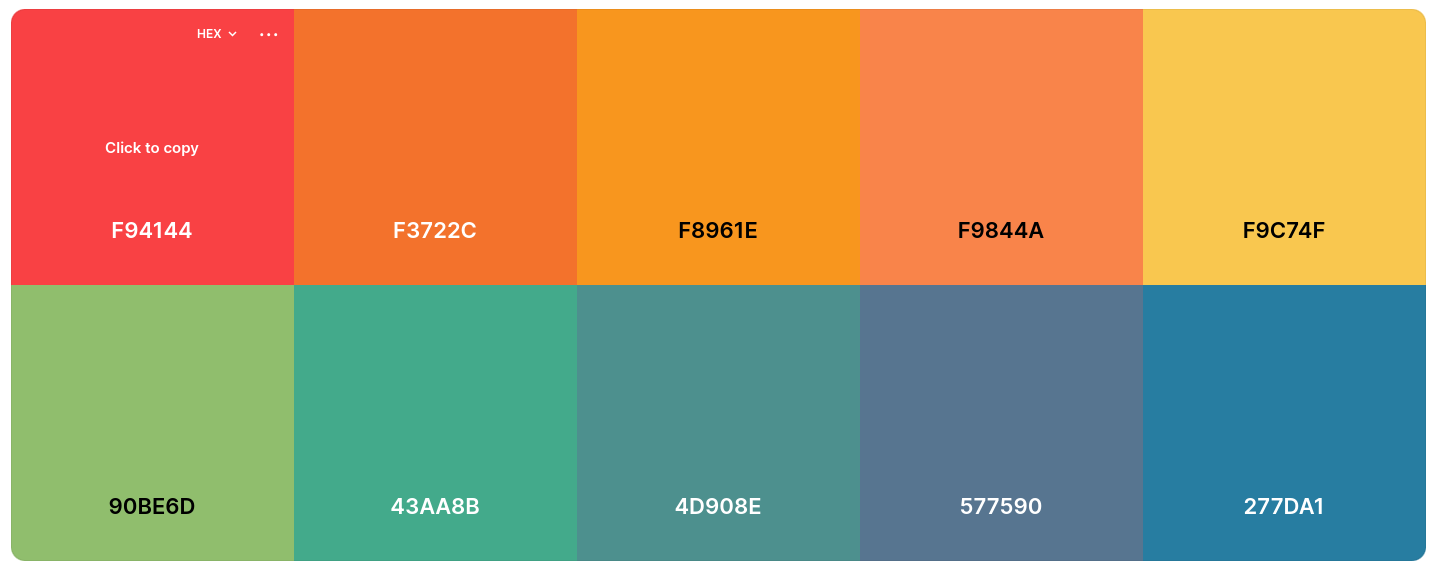
\includegraphics[width=1\textwidth]{USPSC-img/masterPalette.png}
%         \url{https://coolors.co/palette/f94144-f3722c-f8961e-f9844a-f9c74f-90be6d-43aa8b-4d908e-577590-277da1}
%     \end{center}
% \end{figure}